\section{Ford Fulkerson}

\subsection{Sequential Algorithm}
    Ford-Fulkerson (FF) is a greedy algorithm that computes the maximum flow of a graph.  The typical implementation of FF is through using Depth First Search (DFS) in order to continuously augment paths through the residual graph, where an augmenting path is a path of edges in the residual graph with unused capacity greater than 0 from the source to the sink. \cite{FF-Fiset}
    
    The other algorithms described in the other sections are variations based off of FF; however, the goal of this section of the project seeks to parallelize the traditional DFS approach \cite{FFvEk} of FF as other implementations such as Edmond Karp or Dinics takes advantage of specific graph structures.
    \newline
    
    \subsubsection{Pseudo Code of Sequential}
    Note if there are $n$ nodes, each node will be indexed from 0 through $n-1$. In the algorithm, the Source node is indexed as 0 while the Sink node is indexed as $n-1$. See Algorithm~\ref{alg:FFSequential}

    \begin{algorithm}
        \caption{Ford-Fulkerson Pseudo Code}
        \label{alg:FFSequential}
        \begin{algorithmic}[1]
            \Function{augment}{}
                \State $tN \gets sink node$ 
                \State $augNum \gets Integer$ 
            
                \While {$tN$ is not 0}
                    \If{$tN.thisNode$}
                        \State $flow[tN.prevNode][tN.thisNode] \gets$ flow[tN.prevNode][tN.thisNode] + augNum
                    
                    \Else \State $flow[tN.thisNode][tN.prevNode] \gets$ flow[tN.thisNode][tN.prevNode] - augNum
                        
                    \EndIf
                    
                    \State $tN \gets tN$'s previous node
                \EndWhile
            \EndFunction\\\\
    
            \Function{label}{}
                \If {$add:$}
                	\State 
                	    $pFlow \gets$ min(ith-node's potentialFlow, cap[i][j] - flow[i][j])
                \Else
                    \State
    			        $pFlow \gets$ min(ith-node's potentialFlow, flow[j][i])
                \EndIf
            \EndFunction
        \end{algorithmic}
        \begin{algorithmic}[1]
            \State Node:
                \State $prevNode \gets$ Integer
                \State $thisNode \gets$ Integer
                \State $add \gets$ Boolean
                \State $potentialFlow \gets$ Integer\\
                
            
            \State FordFulkerson:
                \State $capacity[][] \gets$ Capacity Graph
                \State $flow[][] \gets$ Flow Graph
                \State $nodeLabels \gets$ Array of Nodes
                \State $numNodes \gets$ Number of nodes in graph\\
                \State $sink \gets$ Integer\\
                
                \For {i in range 2:}
                    \For {i in range numNodes:}
                        \For {j in range numNodes:}
                            \If {jth-node is labeled}
                                \State
                                    \If {ith-node is not labeled and $flow[j][i] < cap[j][i]$}
                                        Label() where $add$ is true
                                    \EndIf
                                    
                                    \If {ith-node is not labeled and $flow[j][i] >$ 0}
                                        Label() where $add$ is false
                                    \EndIf
                            \EndIf
                        \EndFor
                        
                        \If{sink node is labeled}
                            Augment()
                            then do outermost for-loop again
                        \EndIf
                    \EndFor
                \EndFor\\
            \end{algorithmic}
        \end{algorithm}

\subsection{Parallel Algorithm}
        The approach used in a parallel algorithm of Ford-Fulkerson already posed intimidating challenges. Unlike its sibling algorithms, Edmond-Karp in particular, FF is traditionally implemented using DFS, not breadth-first-search (BFS). Without the luxury of an easily-parallelizable algorithm, research had to be done to convert a recursive DFS approach into an iterative one.
        
        During a run of FF, the algorithm attempts to find augmenting paths by conducting two primary steps:
        \begin{enumerate}
            \item Search for a valid flow-augmenting path
            \item Update the flow-augmenting paths on a backward pass
        \end{enumerate}
        
        
        Three options of parallelization were considered during the process of Ford-Fulkerson:
        \begin{enumerate}
            \item Depth-First Search
            \item Augmenting Paths
            \item Backwards Update
        \end{enumerate}
        Attempting to create an iterative version of DFS would have involved the usage of additional overhead in order to simulate recursion, such as the introduction of a stack. For most of the development for this endeavor, the Ford-Fulkerson team had insufficient experience for this.
        
        Rather than navigating through the difficulties of directly turning DFS parallel, a hybrid solution was attempted; the process of traversing a graph's adjacency matrix was combined with labeling the current flow running through the network flow graph. In the end, the attempted solution combines the greedy approach from augmenting the paths by overlapping threads across different connected edges.
        
        
    \subsubsection{Initial Approach}
    
        The adjacency matrix used to represent the flow and the capacity could be parsed in two different ways. Instead of utilizing a traditional row $\xrightarrow{}$ column approach to navigate through the matrix, instead a column $\xrightarrow{}$ row method will be chosen in order to avoid overhead issues that could arise with multiple threads.
    
        
        In the Initial Approach, threads would sweep from left-to-right in the capacity matrix column-by-column. Unfortunately, this particular method of labeling the nodes raises contention issues in the form of multiple threads attempting to acquire a lock. For example, in Figure 1 for the process of labeling the flow from node $A$ to $B$ and $S$ to $B$ causes contention of the labeling of $B$.
        
        
    \subsubsection{Final Approach}
        The chosen parallel approach allows multiple threads to search through the graph's adjacency matrix and interdependently adjust potential flow as all threads traverse the matrix together column-by-column. Utilizing a CyclicBarrier, we implement a wait-free correctness policy as the results of the method calls depend on every single thread successfully reaching that particular bottleneck.
        
        In the Final Approach, threads would sweep from top-to-bottom in the capacity matrix. This is an improvement compared to the Initial Approach 
        since there will be no contention when it comes to labeling a node. This occurs since each thread will attempt to assign a label to a different node.
        
        The work of each thread is load-balanced by having each thread start on a column that are evenly spaced from each other (i.e. if you have 2 threads and a 4x4 capacity, one thread will be on column 0, the other thread will be on column 2.) In other words, this means we can forego the usage of locks, as the threads remain in their respective lanes while traversing the graph for augmenting paths, only stopping to wait for the other threads to get to the CyclicBarrier.
        
        The method of labeling was discovered independently of existing research papers, although not completely novel \cite{Jiang2013APF}, while tracing through simulations of multiple threads augmenting the graph. An important observation was that a single thread must complete this without interruption: once a thread reaches the sink node, it blocks the other threads from augmenting by forcing them to wait at the CyclicBarrier.
    
    \subsubsection{Tracing Through The Final Approach}
        \begin{figure}[h]
            \centering
            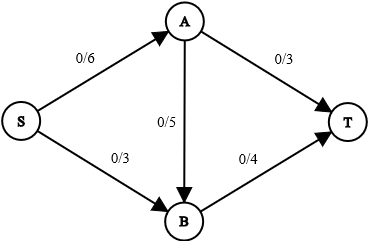
\includegraphics[scale=0.80]{figures/graph.png}
            \caption{Network Flow Graph}
        \end{figure}
    
        \begin{figure}[H]
            \centering
            \[
                \begin{blockarray}{ccccc}
                    & S & A & B & T \\
                    \begin{block}{c(cccc)}
                        S & 0 & 6 & 3 & 0 \\
                        A & 0 & 0 & 5 & 3 \\
                        B & 0 & 0 & 0 & 4 \\
                        T & 0 & 0 & 0 & 0 \\
                    \end{block}
                \end{blockarray}
            \]
            \caption{Adjacency Matrix of Fig. 1's capacity}
        \end{figure}
        
        \begin{figure}[H]
            \centering
            \[
                \begin{blockarray}{ccccc}
                    & S & A & B & T \\
                    \begin{block}{c(cccc)}
                        S & 0 & 0 & 0 & 0 \\
                        A & 0 & 0 & 0 & 0 \\
                        B & 0 & 0 & 0 & 0 \\
                        T & 0 & 0 & 0 & 0 \\
                    \end{block}
                \end{blockarray}
            \]
            \caption{Starting Adjacency Matrix of Fig. 1's flow}
        \end{figure}
        
        Figure 1 and 2 will be used as an example to illustrate how the parallel approach works. There is also another adjacency matrix of the same size as the capacity matrix which keeps track of the flow after augmenting a graph. This flow matrix has a starting state where all the values are initialized to 0. The notation $flow[0][1]$ denotes the element on the 0th row and 1st column of the flow matrix. The notation $cap[0][1]$ denotes the element on the 0th row and 1st column of the capacity matrix (this would be 6 on Figure 2).
        
        
        
        $S$ is the Source node and $T$ is the Sink node. Assume the use of 2 threads $X$ and $Y$. The notation of $X:cap[1][2]$ means thread $X$ is looking at the capacity of 5. Begin all threads in the 0th-index row ($S$). In the actual procedure of the code, the threads would be load-balanced where X is on column 0 and Y is on column 2, but for the sake of quick demonstration, the threads will be on column 1 and 2, respectively.
        
        
        Initially, the threads will be at $X:cap[0][1]$ and $Y:cap[0][2]$ (Note that the Source node column $(cap[\_][0])$ can be skipped since there are no incoming edges to the source node. So the threads can be $X:cap[0][0]$ and $Y:cap[0][1]$ but it is not done here in the example as it is not as helpful for demonstration nor is it efficient). The two threads will then sweep through the rows from top-to-bottom in order to label nodes.
        
        A label will be in the form of a tuple (Ex. ($A$, +, 6)) which respectfully describes: 
            \begin{enumerate}
                \item What node it came from,
                \item What operation (add or subtract) to do when augmenting
                \item The potential flow of the labeled node
            \end{enumerate}
        The Source node is always labeled as (\_, +, $\infty$); once the Sink node is labeled, start the augmentation of the graph by backtracking through the labels of the nodes and use the potential flow labeled on the Sink node when augmenting each of the edges.
        
        A node is only labeled if it is unlabeled in addition to:
        \begin{enumerate}
            \item (Forward Edge) The flow of the edge from previous node (prev) to current node (curr) is less than the capacity from prev to curr.\newline
            For i, j, the indices of the prev node and curr node respectively, $flow[i][j] < cap[i][j]$. This would result in a labeling of (prev, +, min\{$prevPotentialFlow$, $cap[i][j] - flow[i][j]$\}). $prevPotentialFlow$ is simply the third item of the tuple in the label of the previous node.
            \item (Backward Edge) The flow of the edge from the curr node to the prev node is greater than 0.\newline
            For $i$, $j$, the indices of the prev node and curr node respectively, $flow[j][i] > 0$. This would result in a labeling of (prev, -, min\{$prevPotentialFlow$, $flow[j][i]$\})
        \end{enumerate}
        
        Using the rules above:
        \begin{enumerate}
            \item Thread $X$ currently at $X:cap[0][1]$, $X$ will label node $A$ because the previous node $S$ is labeled (with (\_, +, $\infty$)) and $X:flow[0][1] < X:cap[0][1]$. 
            \item  With this, node $A$ will be labeled with ($S$, +, 6).
            \item For thread $Y$ currently at $Y:cap[0][2]$, $Y$ will label node $B$ because the previous node $S$ is labeled and $Y:flow[0][1] < Y:cap[0][2]$.
            \item  Hence, node $B$ will be labeled with ($S$, +, 3). The graph and matrix are shown.
        \end{enumerate}
        
        \begin{figure}[H]
            \centering
            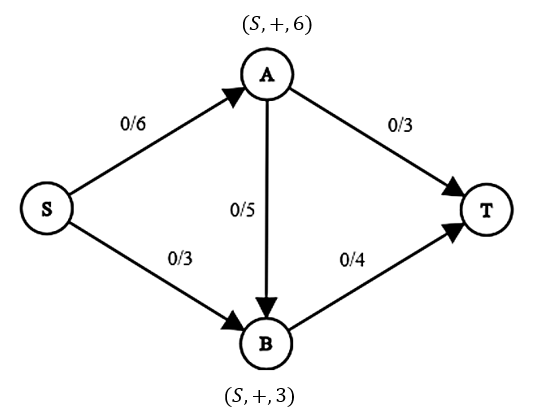
\includegraphics[scale=.5]{figures/nodeAandB.png}
            \caption{Threads $X$ and $Y$ simultaneously labeling nodes $A$ and $B$.}
            \label{fig:Sweep}
        \end{figure}
        \begin{figure}[H]
            \centering
            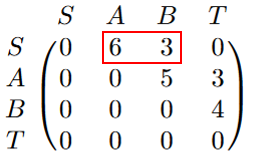
\includegraphics[scale=.5]{figures/Sweep.png}
            \caption{$X:cap[0][1]$ and $Y:cap[0][2]$ on an initial sweep}
            \label{fig:Sweep}
        \end{figure}
        
        After the two threads in this example finish labeling in the 0th-index row, both threads move to the 1st-index row in the same respective column. $X:cap[1][1]$ and $Y:cap[1][2]$ are the next elements the threads will attempt to label. It will be found that $X$ any $Y$ will not label $A$ and $B$ since $A$ and $B$ was already labeled in the previous iteration.
        Hence, the graph in this iteration will look the same as Figure 4.
        
        \begin{figure}[H]
            \centering
            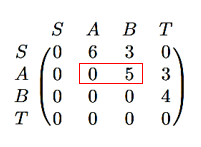
\includegraphics[scale=.7]{figures/Sweep2.png}
            \caption{$X:cap[1][1]$ and $Y:cap[1][2]$ on next sweep}
            \label{fig:Sweep}
        \end{figure}
        
        The threads will continue to sweep down. At the last row, the threads shift over right 1 column and back to the 0th-index for another top-to-bottom sweep. If the threads shift over past the number of columns, it wraps around back to the 0th-index column and continues.

        \begin{figure}[H]
            \centering
            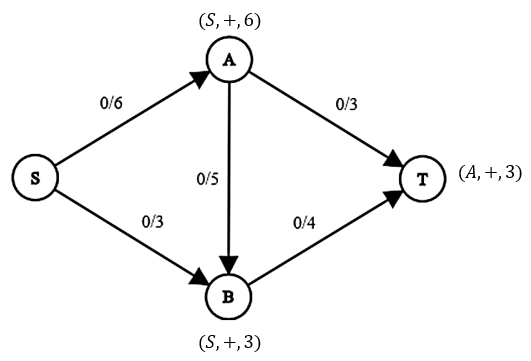
\includegraphics[scale=.6]{figures/hitsink.png}
            \caption{Labeling sink}
            \label{fig:Sweep}
        \end{figure}
        
        \begin{figure}[H]
            \centering
            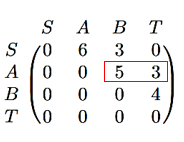
\includegraphics[scale=.7]{figures/cap[1][3].png}
            \caption{$X:cap[1][1]$ and $Y:cap[1][2]$ on sweep}
            \label{fig:Sweep}
        \end{figure}
        
        After an eventual amount of sweeps, the threads go to the 1st-index row ($A$) with $X:cap[1][2]$ and $Y:cap[1][3]$. $Y:cap[1][3]$ will label the Sink node with ($A$, +, 3) once eventually reached. Since the sink is labeled, that thread will backtrack through the graph utilizing the labels as breadcrumbs. Potential flow is added or subtracted based on the 2nd item in the tuple of the label that is currently being scanned. The augmenting ends once the Source node is reached. This was the first augmentation of many that will occur in the graph. Below is the first augmented graph of many.
        
        \begin{figure}[H]
            \centering
            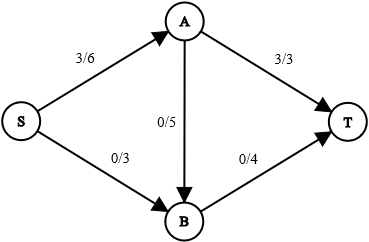
\includegraphics[scale=.7]{figures/FFaugmented.png}
            \caption{The graph after augmenting}
            \label{fig:Sweep}
        \end{figure}
        
        The algorithm continues augmenting the graph until an iteration cannot label any nodes after a top-to-bottom sweep. When the algorithm ends, the maximum flow is found by finding the sum of the flow column of the sink node.
        
        \begin{figure}[H]
            \centering
            \[
                \begin{blockarray}{ccccc}
                    & S & A & B & T \\
                    \begin{block}{c(cccc)}
                        S & 0 & 4 & 3 & 0 \\
                        A & 0 & 0 & 1 & 3 \\
                        B & 0 & 0 & 0 & 4 \\
                        T & 0 & 0 & 0 & 0 \\
                    \end{block}
                \end{blockarray}
            \]
            \caption{Adjacency Matrix of flow after finished algorithm}
        \end{figure}
        
        Hence, the max flow of the graph in this example is 7.
        
    \subsubsection{Pseudo Code of Parallel}
        Note if there are $n$ nodes, each node will be indexed from 0 through $n-1$. The Source node is indexed as 0 while the Sink node is indexed as $n-1$. See Algorithm~\ref{alg:FFParallel}. See Algorithm~\ref{alg:FFSequential} for the Augment and Label functions.
        \begin{algorithm}
            \caption{Ford-Fulkerson Parallel Pseudo Code}
            \label{alg:FFParallel}
            \begin{algorithmic}[1]
                \State Node:
                    \State $prevNode \gets$ Integer
                    \State $thisNode \gets$ Integer
                    \State $add \gets$ Boolean
                    \State $potentialFlow \gets$ Integer\\
                    
                \State FordFulkerson:
                    \State $row \gets$ AtomicInteger
                    \State $capacity[][] \gets$ Capacity Graph
                    \State $flow[][] \gets$ Flow Graph
                    \State $nodeLabels[] \gets$ Array of Nodes
                    \State $numNodes \gets$ number of nodes in graph
                    \State $threadLimit \gets$ Max number of threads
                    \State $tNum \gets$ Identifying Thread number 0-indexed
                    \State $barrier \gets$ CyclicBarrier
                    \\
                    
                    \For {offset in range numNodes:}
                        \State col $\gets$ ((offset * threadLimit) + tNum) \% numNodes
                        \For {$row$ in range numNodes:}
                            \State j $\gets row$
                            \If {jth-node is labeled}
                                \State
                                    \If {node at this col is not labeled and $flow[row][col] < cap[col][row]$}
                                        Label() where $add$ is true
                                    \EndIf
                                    
                                    \If {node at this col is not labeled and $flow[col][row] >$ 0}
                                        Label() where $add$ is false
                                    \EndIf
                            \EndIf\\
                            waitForAllThreadsBeforeProceeding()
                        \EndFor
                        \If{sink node is labeled} \\
                            barrier.wait() // Have threads wait until all arrive\\
                            Only one thread Augment()\\
                            
                            barrier.wait() // Have threads wait until all arrive\\
                            do outermost for-loop again
                        \EndIf\\
                    \EndFor\\
            \end{algorithmic}\\
        \end{algorithm}\\

\subsection{Testing \& Results}
    These test results were performed on UCF's Eustis3 server utilizing open-source data sets \cite{sumitpadhiyar}. The results on the table are an average of 3 runs.
    \newline
    \begin{tabular}{ | m{4em} | m{5em }| m{5em} | m{5em} | } 
      \hline
      Nodes & Max Flow & Sequential Time & Parallel Time \\ 
      
        \hline
        50      & 828     & 5ms & 24ms\\
        \hline
        100     & 1251    & 10ms & 64ms\\  
        \hline
        500     & 7143    & 182ms & 202ms\\        
        \hline   
        750     & 10930   & 396ms & 407ms\\         
        \hline
        1000    & 13476   & 866ms & 790ms\\       
        \hline
        2000    & 25027   & 6532ms & 3848ms\\
        \hline
        3000    & 39170   & 18448ms & 12407ms\\       
        \hline
        4000    & 58517   & 53893ms & 32107ms\\
        \hline
        5000    & 69349   & 117045ms & 52792ms\\
        \hline
        10000   & 142610  & 784219ms & 422210ms\\
        \hline
    \end{tabular}
    
    \begin{figure}[H]
        \centering
        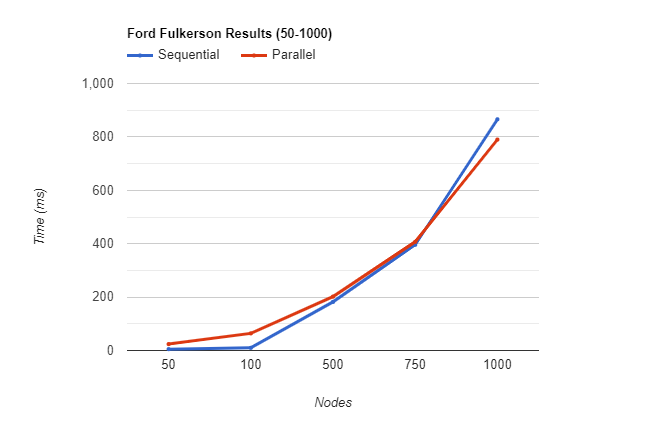
\includegraphics[scale=.48]{figures/low-end-ff.png}
        \label{fig:my_label}
    \end{figure}
    \begin{figure}[H]
        \centering
        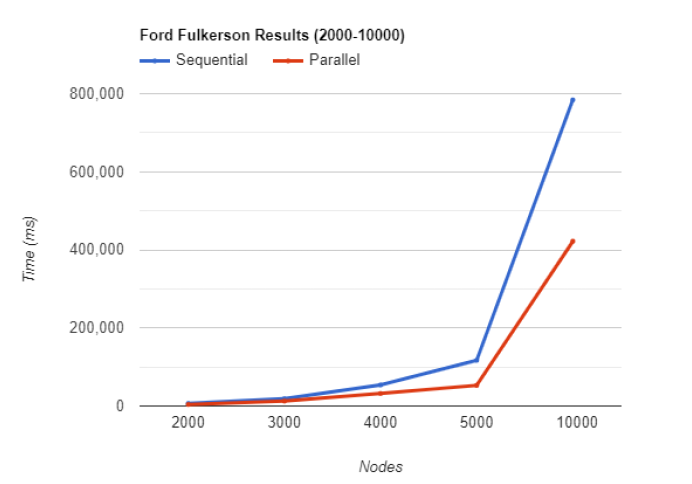
\includegraphics[scale=.48]{figures/high-end-ff.png}
        \label{fig:my_label}
    \end{figure}

    The testing results only begin to show noticeable changes once the node count begins to approach the 500 mark. The parallel implementation of Ford-Fulkerson begins to experience an exponential growth in speed after reaching that threshold, with the 10000 node testcase gaining a 85.74\% increase in speed from the sequential implementation, which is 1.857 times faster. By Amdahl's Law, it can be determined that the parallel program implementation of Ford-Fulkerson is 52.76\% concurrent.
    
    While a parallel implementation of Ford-Fulkerson is viable, from research, practicality it costs more resources than is worth for graph sizes most smaller applications would deal with; from a logical standpoint, creating a parallel Ford-Fulkerson implementation should be more applied to larger use-cases that depend on massive graph sizes.
    
    